\section{Objective 1: \texttt{mpbenchmark}}
As mentioned in the introduction section \texttt{mpbenchmark} performs calculations of a jet engine using multiple threads and produces the time taken to complete these calculations as output. After analysing the code implementation of \texttt{mpbenchmark} the application can be summarised performing the following tasks:

\begin{enumerate}
	\item The application reads data from an input(\texttt{.txt}) file and stores that into an array before starting the calculations. This input data is required to perform calculations required in the next step. 
	\item During calculation, each thread reads input data at specific positions of the input array. After calculation, the results are written into an output array.
	\item In the last step, the benchmark’s response time along with deadlines missed is printed out and saved to an output(\texttt{.txt}) file. 
\end{enumerate}

This design of \texttt{mpbenchmark} can be visualised in figure \ref*{fig:revised_mpbenchmark_structure}.

\begin{figure}[h] % Positioning preference: here, top, bottom, page
	\centering
	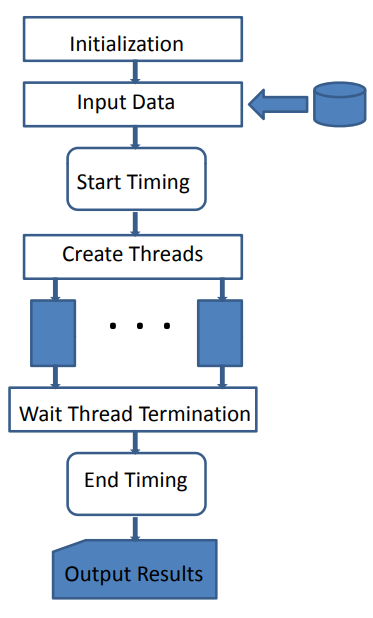
\includegraphics[width=0.5\textwidth, height=10cm]{~/Documents/Part_D_Modules/Individual_Project/Individual_report/figures/revised_mpbenchmark_structure.png} % Adjust the path and width as needed
	\caption{Revised \texttt{mpbenchmark} structure \cite{mpbenchmark_paper}.}
	\label{fig:revised_mpbenchmark_structure} % Use this label to reference the figure
\end{figure}

The source code of \texttt{mpbenchmark} provided a solution in \texttt{C\#}, this served as a useful reference of how figure \ref*{fig:revised_mpbenchmark_structure} would be implemented in code using object-oriented design. Subsequently, the \texttt{C++} object oriented design comprised of three main classes:

\begin{enumerate}
	\item \texttt{FileDataLoader}: the primary function of this class is to load data from the input file and also to allow the user to save output data to the output file.
	\item \texttt{SharedPerformanceData}: this class stores data loaded from the input file into an array and also allows storage of output data into a separate array. But importantly it allows threads to access specific parts of the input data in a thread-safe manner. 
	\item \texttt{Worker}: this class contains functions to perform the important calculations, computations of deadlines missed and output data. This class defines the \texttt{operator ()} which encapsulates the main calculations, this class design is know as a \texttt{Functor}.
\end{enumerate}

The \texttt{C++} object-oriented class design can be visualised using a UML class diagram shown in figure \ref*{fig:mpbenchmark_UML_diagram}.

\begin{figure}[h] % Positioning preference: here, top, bottom, page
	\centering
	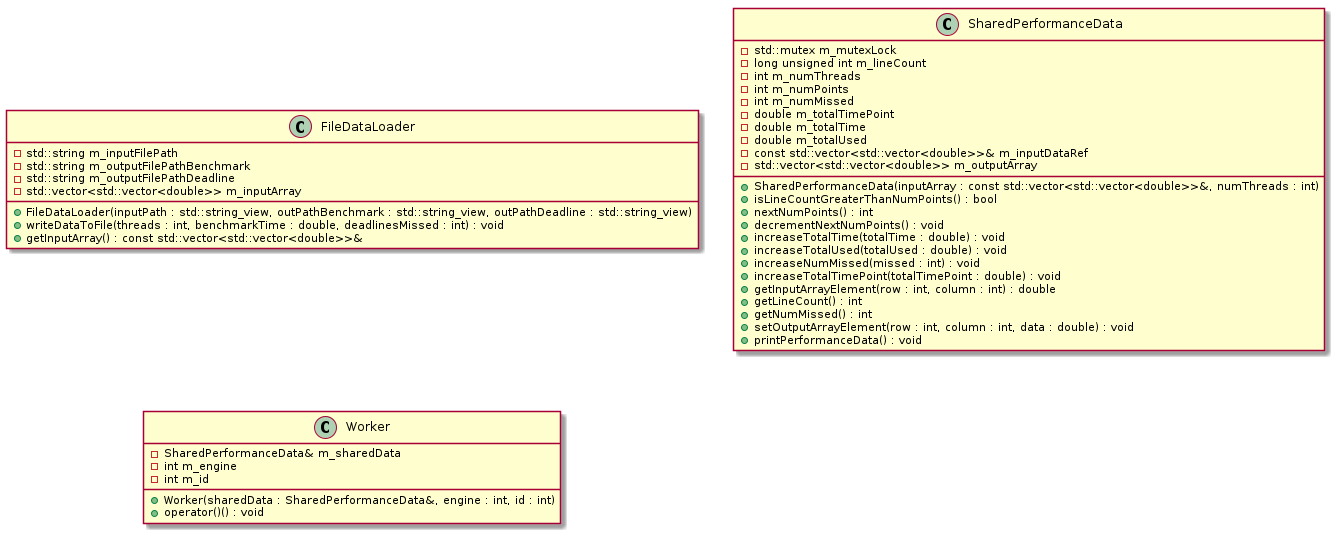
\includegraphics[width=1\textwidth, height=60cm]{~/Documents/Part_D_Modules/Individual_Project/Individual_report/figures/mpbenchmark_class.png} % Adjust the path and width as needed
	\caption{UML class diagram of the proposed \texttt{C++} solution.}
	\label{fig:mpbenchmark_UML_diagram} % Use this label to reference the figure
\end{figure}

These classes are used in the following sequence in the proposed solution[insert UML sequence diagram]:

The \texttt{mpbenchmark} implementation in the \texttt{C} language utilized the \texttt{printf} function for output throughout the application. Transitioning this functionality to \texttt{C++} posed a challenge, as \texttt{printf} relies on ``format string based" formatting, whereas \texttt{C++} typically uses ``stream-based" formatting through \texttt{std::cout}. This discrepancy was addressed in the \texttt{C++20} standard with the introduction of \texttt{std::format}. However, oddly enough, \texttt{std::format} was not supported by the \texttt{gcc} compiler version on the target system, despite it supporting the \texttt{C++20} standard\cite{std_format_gcc_compiler_version}. A workaround involved using the \texttt{fmt::print} function from the \texttt{fmt} library, which is noted as the inspiration behind \texttt{std::format}\cite{fmt_printing_library}. Detailed system specifications and a code snippet demonstrating the use of \texttt{fmt::print} are provided in the appendix.

The original \texttt{mpbenchmark} code included a command line argument allowing the user (or developer) to specify the engine type for computations. The application supports three distinct engine types. Importantly, the number of threads the application employs can be modified using the \texttt{taskset} command in \texttt{Linux}, which determines the CPU cores the application can run on. To improve this functionality, a second command line argument was added in the proposed solution. This new parameter enables users to set the number of threads the application should use. If this argument is omitted, the application automatically defaults to the maximum number of threads available on the system. This enhancement is detailed in a code snippet in the appendix.

To compile and link the application, the industry standard \texttt{CMake}\cite{cmake_about} software was used. In the \texttt{CMakeLists.txt}(the file used for building the project), the key aspects were specifying the \texttt{C++20} standard, including the \texttt{fmt} library and compilation with the \texttt{-O2} flag. This optimisation flag was also used by the authors of \texttt{mpbenchmark}\cite{mpbenchmark_paper} therefore it was used in the proposed solution for consistency. 

To further enhance the performance of the \texttt{mpbenchmark}, the \texttt{Valgrind/Callgrind} function profiler tool was deployed to find potential bottlenecks. \texttt{Callgrind} profiling results showed that part of the application where it approximates the value of $\pi$ had the highest self-cost. This code snippet is shown in the listing ~\ref{lst:pi_approximation_1} below:

\begin{lstlisting}[
	caption={Part of the code with the highest self-cost. It approximate $\pi$ using numerical integration.},
	label={lst:pi_approximation_1}
	]
// initialise variables for the pi calculation
const long num_steps = 1000000;
double step = 1.0 / static_cast<double>(num_steps);
double x{}, pi{}, sum{};

// performing numerical integration using the midpoint Riemann sum
for (int i = 0; i < num_steps; i++) {
	x = (i + 0.5) * step;
	sum += 4.0 / (1.0 + x * x);
}
pi = sum * step;
\end{lstlisting}

The problem with this part of the code is that it already part of the parallel regions where it is executed by each thread. It may seen like a good candidate for applying parallel \texttt{for loop} from the OpenMP library however creating nested threads beyond the number of threads available on the system does not always lead to higher performance and in many cases can degrade performance. Another way to improve performance is by using SIMD intrinsics, this a programming tool to improve single-threaded or sequential performance of a code it stands for ``Single Instruction Multiple Data". By using these intrinsics, programmers can write code that processes data in parallel directly within a single CPU cycle. An advantage of using \texttt{C++}(and/or \texttt{C}) is that SIMD intrinsics can be deployed whereas higher level languages like \texttt{Java} or \texttt{C\#} make it very difficult to access these. 

SIMD intrinsics vary by the target CPU, \texttt{x86} processors (which are found in most laptop and desktops) use \texttt{AVX2} instructions whereas \texttt{ARM} processors(commonly found in Apple products and embedded devices) use \texttt{NEON} instructions. In this project we need to use both as our proposed \texttt{C++} solution will be deployed on both desktop(\texttt{x86} processor) and Raspberry Pi devices(\texttt{ARM} based processor). The SIMD enhanced code can be summarised algorithmatically in the following steps and shown as a code snippet in listing ~\ref{lst:pi_approximation_2}: 

\begin{enumerate}
	\item Initialise \texttt{256-bit} wide vectors: each vector can hold four double-precision (\texttt{64-bit}) floating point numbers. The main initialisations would be a vector to hold four loop indices (\texttt{vec\_i}), a vector to calculate four values of $x$ (\texttt{vec\_x}), a vector to hold the result of the integrand (\texttt{vec\_temp}) and a vector to accumulate the sum (\texttt{vec\_sum}) after each loop iteration.
	\item \texttt{for loop} iterate until \texttt{num\_steps/4}:
	\begin{itemize}
		\item step 1: calculate the four midpoints $x$-values simultaneously using the vector \texttt{vec\_i} and hold result in \texttt{vec\_x}. Original formula used: \texttt{(i + 0.5) * step}.
		\item step 2: compute the value of the integrand in parallel using the four calculated $x$-values stored in \texttt{vec\_x}, store result in \texttt{vec\_temp}. Original formula used: \texttt{4 / (1 + x * x)}.
		\item step 3: accumulate the values from \texttt{vec\_temp} into the \texttt{vec\_sum} vector.
		\item step 4: increment loop indices vector \texttt{vec\_i} by \texttt{4}. 
	\end{itemize}
	\item Final summation: upon the completion of the loop, perform a horizontal sum on the vector (\texttt{vec\_sum}) that held the accumulated values.
	\item Calculation of $\pi$: sum is multiplied by the step size to approximate the value of $\pi$. Original formula used : \texttt{pi = sum * step}.
\end{enumerate}

The SIMD enhanced code implemented using \texttt{AVX2} instructions of listing ~\ref{lst:pi_approximation_1} is shown below in listing ~\ref{lst:pi_approximation_2}: 

\begin{lstlisting}[
	caption={SIMD enhanced code for approximation of $\pi$ using \texttt{AVX2} instructions. (Horizontal sum function in line 28 can be found in appendix).},
	label={lst:pi_approximation_2}
	]
double Worker::approximatePi(){
	double pi = 0.0; // Initialize pi to 0.0
	static constexpr long num_steps = 1000000; 
	static constexpr double step = 1.0 / static_cast<double>(num_steps); 
	
#if defined(__AVX2__)
	// Use AVX2 SIMD instructions if available
	double sum = 0; // Initialize scalar sum to accumulate final result
	
// Initialise all necessary 256-bit vectors
	__m256d vec_sum = _mm256_set1_pd(0.0);
	__m256d vec_step = _mm256_set1_pd(step);
	__m256d vec_half_step = _mm256_set1_pd(0.5 * step); 
	__m256d vec_one = _mm256_set1_pd(1.0); 
	__m256d vec_four = _mm256_set1_pd(4.0); 
	__m256d vec_x, vec_temp; 
	__m256d vec_i = _mm256_set_pd(3, 2, 1, 0); 
	__m256d vec_increment = _mm256_set1_pd(4); 

// Perform 4 computations at once, note "i" is incremented by 4 instead of 1
	for (int i = 0; i < num_steps; i += 4) {
		vec_x    = _mm256_add_pd(_mm256_mul_pd(vec_i, vec_step), vec_half_step); 
		vec_temp = _mm256_div_pd(vec_four, _mm256_add_pd(vec_one, _mm256_mul_pd(vec_x, vec_x))); 
		vec_sum  = _mm256_add_pd(vec_sum, vec_temp); 
		vec_i    = _mm256_add_pd(vec_i, vec_increment); 
	}
// Perform horizontal sum on vec_sum to get a scalar sum
	sum = hsum256_pd(vec_sum);
 // Multiply the sum by the step size to approximate pi
	pi = sum * step; 

#else
// If AVX2/SIMD instructions are unavailable then resort to using regular code... 
#endif

	return pi; 
}
\end{lstlisting}

As discussed, to utilize SIMD intrinsics on Raspberry Pi devices, \texttt{NEON} instructions must be employed. \texttt{NEON} instructions come with limitations, notably in their support for double precision floating points, which is restricted, and their vector width, which is only \texttt{128-bit}, compared to the \texttt{256-bit} vectors seen in \texttt{AVX2}\cite{neon_reference}. To accommodate \texttt{NEON}, two solutions were developed: one using single precision floating points (\texttt{float}) and the other using double precision floating points (\texttt{double}). The \texttt{NEON} code with \texttt{float} can perform four computations simultaneously, while the code with \texttt{double} can manage only two computations simultaneously, due to the \texttt{128-bit} vector's capacity to store four \texttt{float} values or two \texttt{double} values. Typically, \texttt{float} variables offer less decimal precision than \texttt{double} variables. These two SIMD-enhanced solutions, along with their decimal accuracy levels, will be compared in the results and discussion section. The \texttt{NEON} implementation follows the same algorithm as the code snippet shown in Listing~\ref{lst:pi_approximation_2}, and is available in the appendix.

In summary, for desktop (\texttt{x86}) processors, two main solutions have been developed: a novel \texttt{C++} solution and a SIMD-enhanced \texttt{C++} solution as discussed in Listing~\ref{lst:pi_approximation_2}. For the Raspberry Pi devices, three solutions have been created: the first is the novel \texttt{C++} solution, identical to that on the desktop, and the other two are the SIMD-enhanced versions utilizing \texttt{NEON} instructions with single and double precision floating point variables.

\section{Objective 2: \texttt{MobileNet}}
\section{Objective 3: \texttt{DeBaTE-FI platform}}